\documentclass[]{article}
\usepackage{lmodern}
\usepackage{amssymb,amsmath}
\usepackage{ifxetex,ifluatex}
\usepackage{fixltx2e} % provides \textsubscript
\ifnum 0\ifxetex 1\fi\ifluatex 1\fi=0 % if pdftex
  \usepackage[T1]{fontenc}
  \usepackage[utf8]{inputenc}
\else % if luatex or xelatex
  \ifxetex
    \usepackage{mathspec}
  \else
    \usepackage{fontspec}
  \fi
  \defaultfontfeatures{Ligatures=TeX,Scale=MatchLowercase}
\fi
% use upquote if available, for straight quotes in verbatim environments
\IfFileExists{upquote.sty}{\usepackage{upquote}}{}
% use microtype if available
\IfFileExists{microtype.sty}{%
\usepackage{microtype}
\UseMicrotypeSet[protrusion]{basicmath} % disable protrusion for tt fonts
}{}
\usepackage[margin=1in]{geometry}
\usepackage{hyperref}
\hypersetup{unicode=true,
            pdftitle={RGR MS},
            pdfauthor={Chris H. Wilson},
            pdfborder={0 0 0},
            breaklinks=true}
\urlstyle{same}  % don't use monospace font for urls
\usepackage{graphicx,grffile}
\makeatletter
\def\maxwidth{\ifdim\Gin@nat@width>\linewidth\linewidth\else\Gin@nat@width\fi}
\def\maxheight{\ifdim\Gin@nat@height>\textheight\textheight\else\Gin@nat@height\fi}
\makeatother
% Scale images if necessary, so that they will not overflow the page
% margins by default, and it is still possible to overwrite the defaults
% using explicit options in \includegraphics[width, height, ...]{}
\setkeys{Gin}{width=\maxwidth,height=\maxheight,keepaspectratio}
\IfFileExists{parskip.sty}{%
\usepackage{parskip}
}{% else
\setlength{\parindent}{0pt}
\setlength{\parskip}{6pt plus 2pt minus 1pt}
}
\setlength{\emergencystretch}{3em}  % prevent overfull lines
\providecommand{\tightlist}{%
  \setlength{\itemsep}{0pt}\setlength{\parskip}{0pt}}
\setcounter{secnumdepth}{0}
% Redefines (sub)paragraphs to behave more like sections
\ifx\paragraph\undefined\else
\let\oldparagraph\paragraph
\renewcommand{\paragraph}[1]{\oldparagraph{#1}\mbox{}}
\fi
\ifx\subparagraph\undefined\else
\let\oldsubparagraph\subparagraph
\renewcommand{\subparagraph}[1]{\oldsubparagraph{#1}\mbox{}}
\fi

%%% Use protect on footnotes to avoid problems with footnotes in titles
\let\rmarkdownfootnote\footnote%
\def\footnote{\protect\rmarkdownfootnote}

%%% Change title format to be more compact
\usepackage{titling}

% Create subtitle command for use in maketitle
\newcommand{\subtitle}[1]{
  \posttitle{
    \begin{center}\large#1\end{center}
    }
}

\setlength{\droptitle}{-2em}
  \title{RGR MS}
  \pretitle{\vspace{\droptitle}\centering\huge}
  \posttitle{\par}
  \author{Chris H. Wilson}
  \preauthor{\centering\large\emph}
  \postauthor{\par}
  \predate{\centering\large\emph}
  \postdate{\par}
  \date{March 2, 2019}


\begin{document}
\maketitle

\subsubsection{Background and Rationale}\label{background-and-rationale}

Analyzing growth of individuals is fundamental in many areas of ecology
and biology. A common situation is the need to intercompare multiple
individuals across genotypes or species in experimental or observational
settings where variations in initial sizes and environmental factors
both contribute to observed variations in size at any point in time. In
this setting, a common default practice is to re-express growth as a
relative measure, dividing the growth increment by the initial size. In
the limit as the time period goes to zero, this can be represented as
\[\frac{dS}{dt}\frac{1}{S}\]

Without explicit specification of a time-varying dynamic, e.g.~some kind
of non-linear growth function, this representation corresponds to
exponential growth. That is, the quantity obtained by integration of
\[\frac{dS}{dt}\frac{1}{S} = k\] over some time period, and given some
initial size \(S_0\)

is simply the familiar exponential equation \[S_t = S_0e^{kt}\]

The quantity in equation 1 is often referred to as relative growth rate
(RGR), and the usual method of quantification, hereafter the ``log
measure'' corresponds to the solution in 2, as is readily checked. The
log measure is, simply \(\frac{log(S_2) - log(S_1)}{t}\)

The log measure is very frequently utilized as a default in place of
taking the simply difference \(\frac{S_2 - S_1}{t}\). XXX et al. (2012)
summarized several flaws of the log measure and recommended instead to
fit non-linear growth functions. I wholeheartedly concur with this
advice. However, ecologists are often confronted with datasets where
only 2 or 3 time periods are available, thus precluding effective
fitting of non-linear functions.

In this note, I demonstrate that the log measure should also not be used
in the data limited setting of only 2 or 3 observation times. Instead,
the linear difference is to be preferred for three reasons: 1)
simplicity of interpretation, 2) ecological/biological validity, and 3)
ease of use.

\subsubsection{Conceptual Overview}\label{conceptual-overview}

First, we assume a basic theoretical framework for growth: the sigmoidal
curve. Nearly every biologically motivated growth model follows
sigmoidal behavior. For instance, West et al. (2001) famously derived a
sigmoidal equation for growth from metabolic scaling theory. Although
the universality of their particular model has been challenged,
saturating non-linear growth has not. Therefore, we will compare the
linear difference and the log measure to a sigmoidal curve, which is
itself presumed to better approximate underlying biological/ecological
reality. Before proceeding to a brief mathematical exposition, let's
consider a heuristic/intuitive argument. The following figure
encapsulates my entire argument:

\begin{figure}
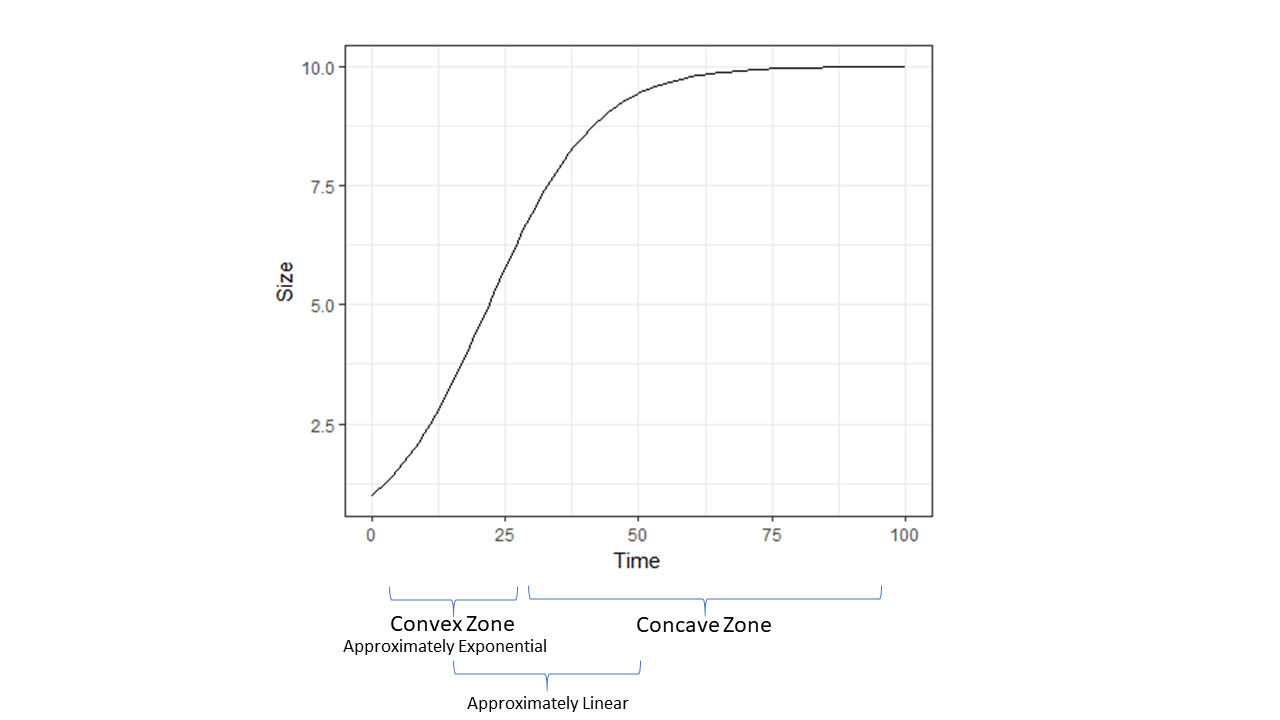
\includegraphics[width=1\linewidth]{Conceptual_Fig} \caption{Conceptual Argument}\label{fig:unnamed-chunk-2}
\end{figure}

In the convex zone, the usual log measure is a fine approximation.
However, the zone of approximate linearity is just as large (if not
larger), where the linear difference is to be preferred. Finally,
neither approximation is great in the upper portion of the concave zone,
although as demonstrated below, the linear approximation is uniformly
superior there.

Mathematically, the argument can be boiled down for any generic equation
for growth over time: \(S_t = f(S,t)\). Using Taylor Series, we can
approximate around some value \(a\) to second order with a generic
function \(g(S,t)\) as:
\[f(S,t) \approx g(S=a,t) + g'(S=a,t) \times (S-a) + \frac{1}{2}g''(S=a,t)\times(S-a)^2\]

As noted above, the canonical log measure corresponds to exponential
dynamics \(S_t = S_0e^{kt}\). Use of exponential dynamics to approximate
\(S_t = f(S,t)\) obviously only works well where both the first and
second derivative of \(f(S,t)\) are positive (i.e.~where function is
convex). Given that the second derivative of any sigmoidal curve flips
from positive to negative, this approximation error grows rapidly
outside of a narrow zone.

\subsubsection{Mathematical Analysis of Log
Measure}\label{mathematical-analysis-of-log-measure}

We take the familiar logistic equation as a reasonable representaton for
sigmoidal growth, while noting that many options are available:

\[S_t = \frac{KS_0e^{rt}}{K+P_0(e^{rt}-1)}\]

Given this representation of underlying growth, the first question is:
what does the canonical log measure \(\frac{log(S_2) - log(S_1)}{t}\)
correspond to? In other words, we want to ask what happens given exact
measurements of \(S_2\) and \(S_1\), given that they are sampled from
above equation. For \(log(S_t)\) We have:

\[\log(S_t) = log(K) + log(S_0) + rt - log(K + S_0(e^{rt}-1))\]

If we have size observations \(S_1\) and \(S_2\) from two times, \(t_1\)
and \(t_2\),the difference between them is:

\[\log(S_2) - log(S_1) = r(t_2 - t_1) + log(\frac{K + P_0(e^{rt_1}-1)}{K + P_0(e^{rt_2}-1)})\]

For any given interval \(t_2~t_1\):\\
\[\frac{log(S_t) - log(S_0)}{t_2 - t_1} = r + \frac{1}{t_2-t_1}log(\frac{K + P_0(e^{rt_1}-1)}{K + P_0(e^{rt_2}-1)})\]
One flaw of the canonical log measure (as pointed out previously by
XXXX) is that it is really time-varying, but in effect treated as though
time constant (by necessity given the limitation of data). If we want to
investigate how this quantity varies with sampling of arbitrary
timepoints \(t_2\) and \(t_1\) along the sigmoidal curve, we re-express
\(t_2=t_1+\Delta\) and let \(t_1=t\)
\[\frac{log(S_{t+\Delta}) - log(S_t)}{\Delta} = r + \frac{1}{\Delta}log(\frac{K + P_0(e^{rt}-1)}{K + P_0(e^{r({t+\Delta})}-1)})\]

Graphically, the comparison with the observed growth increments is:
\includegraphics{Growth_Measure_MS_files/figure-latex/unnamed-chunk-3-1.pdf}

This comparison, while visually striking, is fundamentally misleading
since the log measure does not really have the same dimensions as the
observed growth increment. It is really a \textbf{rate} with dimensions
of \(\frac{1}{time}\), and the usual re-expression as \(g~g^-1~time^-1\)
is unhelpful at best. Thus, the only way to compare use of the canonical
log measure to the simple linear measure is to reformulate the problem
in terms of implied dynamics.

\subsubsection{Comparing log measure and linear measure in terms of
dynamics}\label{comparing-log-measure-and-linear-measure-in-terms-of-dynamics}

Use of the linear difference \(\frac{S_2 - S_1}{t}\) corresponds to
assumption of a static linear growth rate dynamic, just as use of
\(\frac{log(S_2) - log(S_1)}{t}\) corresponds to assuming a static
exponential growth rate dynamic. In the latter case, the log-measure has
the nice property of representing an ergodic observable (sense Peters
and Gell-man 2016). While widely (and rightly) dismissed as unrealistic,
the linear dynamic \(\frac{S_2 - S_1}{t}\) may in fact be a generally
superior measure for ecological analysis where no time series of
size/biomass data is available.

The comparison made here is the goodness of fit implied by replacing the
sigmoidal \(S_t\) with either a linear approximation or an exponential
approximation, given sampling of size from two pairs of time points: 1)
from the early (``exponential'') portion of sigmoid curve, and 2) from
the middle (``linear'') portion of sigmoidal curve, and 3) from the
saturating part of curve.

\begin{enumerate}
\def\labelenumi{\arabic{enumi})}
\tightlist
\item
  \(t_2 = 14\) and \(t_1=2\):
\end{enumerate}

\begin{verbatim}
## Warning: Removed 33 rows containing missing values (geom_path).
\end{verbatim}

\includegraphics{Growth_Measure_MS_files/figure-latex/unnamed-chunk-4-1.pdf}
As expected, the exponential approximation works better with data from
the convex portion of growth curve. However, the improvement is marginal
in absolute value, and quickly diverges outside of the convex portion
(in accord with our intuitive model).

\begin{enumerate}
\def\labelenumi{\arabic{enumi})}
\setcounter{enumi}{1}
\tightlist
\item
  \(t_2 = 25\) and \(t_1 = 12\):
\end{enumerate}

\begin{verbatim}
## Warning: Removed 18 rows containing missing values (geom_path).
\end{verbatim}

\begin{verbatim}
## Warning: Removed 2 rows containing missing values (geom_path).
\end{verbatim}

\includegraphics{Growth_Measure_MS_files/figure-latex/unnamed-chunk-5-1.pdf}
As can be seen, the linear model is a better approximation where data
are taken from within the center part of the growth cycle. Again, the
improvement is marginal, but real. Forecast accuracy is much higher, and
backcast accuracy marginally worse.

\begin{enumerate}
\def\labelenumi{\arabic{enumi})}
\setcounter{enumi}{2}
\tightlist
\item
  \(t_2=45\) and \(t_1=30\)
\end{enumerate}

\includegraphics{Growth_Measure_MS_files/figure-latex/unnamed-chunk-6-1.pdf}
As expected, in this scenario, the linear approximation is uniformly
better and thus always to be preferred.

\subsubsection{Statistical Properties}\label{statistical-properties}

We can derive the sampling distribution of the log measure
\(\frac{log(S_2) - log(S_1)}{t}\) based on a Taylor Series'
approximation. Specifically, we consider measurements \(S_2\) and
\(S_1\) with normally distributed error, where the variance scales with
the mean (a fairly typical property in biological/ecological data). The
distribution of \(S_2\) - \(S_1\) is then simply the difference of two
Normals. Next, we approximate the moments of the distribution of
\(log(S_t)\) as:
\[E[log(S_t)] \approx log(\mu_{S_t}) - \frac{\sigma^2}{2*\mu_{S_t}^2}\].
Using the delta method for variance, we have:
\[Var[log(S_t)] \approx \frac{\sigma^2}{\mu_{S_t}^2}\]

Given a constant coefficient of variation (reflecting variance scaling
with mean on the original scale) \(CV_s\) the sampling distribution of
\(\frac{log(S_2) - log(S_1)}{t}\) (setting \(t\) to unit scale), is
therefore: \[ N(log(S_2) - log(S_1), \sqrt2CV_s)\]

The CV of the log measure is then related to the expectaiton of the Z
scores of the new sampling distribution, and is inversely proportional
to statistical power: \[CV_l =\frac{\sqrt2}{log(S_2) - log(S_1)}CV_s\]

Thus, where \(log(S_2) - log(S_1) > \sqrt2\) over a unit time increment,
the log measure should have greater statistical power, while it loses
statistical power as the log measure declines (which as we saw in
section XXX above occurs faster than the linear difference of course).
This can be reformulated as \(S_2=S_1e^{\sqrt2}\), revealing a
\emph{scale free} property of statistical analysis of the log measure.
Specifically, wherever the multiplicative growth increase on a unit time
scale \(<e^{\sqrt2}\), the log measure has worse statistical properties
than the linear difference.

For our previous parameter value simulations above, here is the curve of
\(CV_l\) with time \(t\), expressed in multiples of \(CV_s\):
\includegraphics{Growth_Measure_MS_files/figure-latex/unnamed-chunk-7-1.pdf}

As can be seen, in this situation, it is always worse! What happens if
we accelerate growth rate considerably (5X)

\includegraphics{Growth_Measure_MS_files/figure-latex/unnamed-chunk-8-1.pdf}

There is a small window in early growth where it is expected to have
better properties for estimating observed differences, but it rapidly
loses power.

\subsubsection{Case Study: A Situation Statistical Analysis of Log
Measure and Linear Measure
Diverge}\label{case-study-a-situation-statistical-analysis-of-log-measure-and-linear-measure-diverge}

Maybe not necessary here. Theoretical demonstration feels complete.

\subsubsection{Conclusions and
Recommendations}\label{conclusions-and-recommendations}

In summary, the chief virtue of the \(\frac{log(S_2) - log(S_1)}{t}\)
measure is that it effectively linearizes the differences in size from
the convex portion of biological growth curve. Thus, it arguably might
increase the ability to infer subtle but consequential differences in
growth rates based on small differences in observed sizes. However,
analysis of the statistical sampling distribution suggests that
inference on this quantity is actually more difficult than inference on
the linear measure. In fact, ability to detect differences rapidly
declines with position on the sigmoidal curve.

The much maligned linear measure is a superior default on three grounds
therefore. First, it corresponds far more directly with current
ecological reality. It is a measure with an interpretable biological
dimension (usually mass or length, whereas the log measure has
dimensions of \(\frac{1}{time}\)). This enables us to more literally
describe our system. Second, interpreted in terms of dynamics, it is
\emph{less wrong} than the exponential approximation implied by the log
measure. Third, it has superior statistical properties almost
everywhere.

The widespread use of the log measure of ``RGR''
\(\frac{log(S_2) - log(S_1)}{t}\) as an \emph{a priori} preferred
default for the data-limited situation should be abandoned. Where only
two or three time points are available, fitting a linear growth trend is
just as good if not better than estimating an exponential growth rate.
The ideal scenario is to collect a proper time series (5-7+) and fit a
proper growth model. Where data are at all limiting, we recommend
careful incorporation of literature values and other external
information as priors in a fully Bayesian analysis in order to
regularize inferences.


\end{document}
